\section{Physical Layer}

\subsection{Begriffe}

\subsubsection{(Leitungs-)Symbol}
Zu einem gewissen Zeitpunk übertragenes physikalisches Signal das mit einer
bestimmten Symbolrate seinen Wert verändert.

\textcolor{red}{nicht wie in INCO ''eine von N möglichen Nachrichten''}

\subsubsection{Informationsgehalt/Bit}
Informationsgehalt (von Symbol/Nachricht)
$ N_{Bit} = ld(\text{Anzahl Möglichkeiten}) $

\subsubsection{Zeichen}
Einheit der übetragenen Daten, z.B. ein ASCII Zeichen

\subsubsection{Baudrate}
Schrittgeschwindigkeit = Leitungs-Symbole pro Sekunde

Maximale Baudrate $f_s$ ist doppelte Bandbreite $B$ (Hz) gemäss Nyquist:
$$f_s = 2B$$

\subsubsection{Durchsatz/Bit-/Datenübertragungsrate}
übertragung von Information pro Zeit

Maximale Bitrate (Hartley's Gesetz)
$$R \le 2B * ld(\text{\#unterscheidbare Signalzustände})$$

Potenzen (in der Kommunikation werden NICHT zweierpotenzen verwendet):
\begin{itemize}
    \item kBit = $10^3$ Bit $\rightarrow$ kbps = $10^3$ bps
    \item MBit = $10^6$ Bit $\rightarrow$ Mbps = $10^6$ bps
    \item GBit = $10^9$ Bit $\rightarrow$ Gbps = $10^9$ bps
\end{itemize}

\subsubsection{Kanalkapazität}
Berücksichtigt neben der Bitrate auch Störungen
$$C_s [Bit/s] = B * ld(1 * \frac{S}{N})$$

\subsubsection{Verkehrsbeziehung und Kopplung}
\begin{center}
    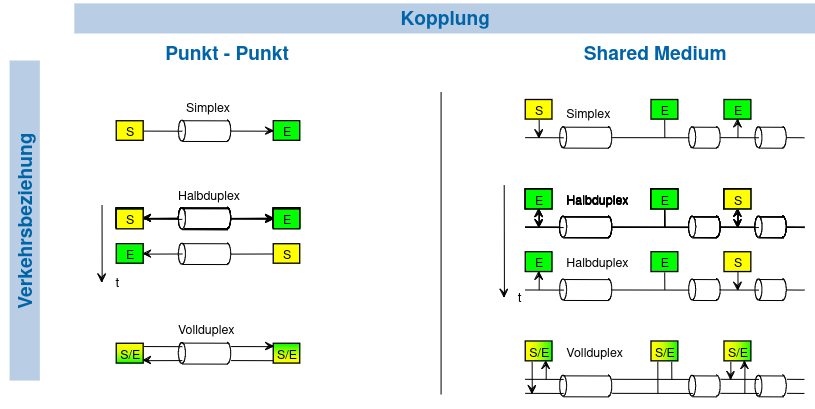
\includegraphics[width=0.9\linewidth]{verkehrsbeziehung-kopplung}
\end{center}

\subsection{Leitungscodes}
Anforderungen:
\begin{itemize}
    \item Takt sollte im Signal enthalten sein (Taktrückgewinnung)
    \item effiziente Bandbreitennutzung
    \item möglichst gleichspannungsfrei (um Sender \& Empfänger mit z.B.
          Transformatoren galvanisch trennen zu können)
\end{itemize}


\subsubsection{3-wertiger AMI (Alternate Mark Inversion)}
Wechsel +/- bei jeder 1 sonst 0 $\rightarrow$ +/- gleichen sich aus
somit Gleichspannungsfrei
\begin{center}
    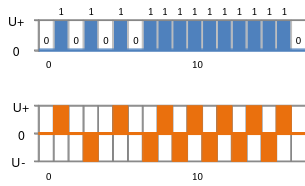
\includegraphics[width=0.8\linewidth]{ami-3}
\end{center}

\subsubsection{PAM3}
Anwendung bei 10 Mbit/s Ethernet via Single Pair bis 1.2km
\begin{itemize}
    \item 4 Bit werden zu 3 ternären Symbolen
    \item DC/Gleichspannungs Offset wird bei Codierung berücksichtigt
\end{itemize}

\subsubsection{Manchester-Code}
Einsatz bei 10BASE-T (Pegel dort +2.5V bis -2.5V)\\
Einfache Codierung: 1 werden als steigende Flanke, 0 als fallende Flanke übertragen.
Signalwechsel bei jedem Bit $\rightarrow$ einfache Taktrückgewinnung

\subsubsection{NRZI (Non Return to Zero Inverted)}
Einsatz bei 100BASE-TX(mit zusätzlicher 4 zu 5 bit codierung)
\begin{center}
    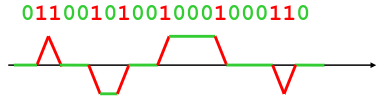
\includegraphics[width=0.9\linewidth]{nrzi}
\end{center}

\subsubsection{RS232}
\begin{center}
    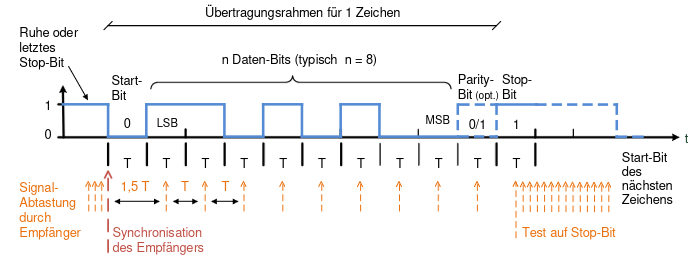
\includegraphics[width=0.9\linewidth]{rs232}
\end{center}






